\documentclass[12pt,a4paper]{article}

% Türkçe %
\usepackage[utf8]{inputenc} %Türkçe karakterler için
\usepackage[T1]{fontenc}
\renewcommand{\tablename}{Tablo}
\renewcommand{\figurename}{Şekil}
\renewcommand{\indexname}{Dizin}
\renewcommand{\listfigurename}{Şekiller}
\renewcommand{\listtablename}{Tablolar}
\renewcommand{\contentsname}{İçindekiler}
\setcounter{tocdepth}{4}
\setcounter{secnumdepth}{4}
% Türkçe %

\usepackage{geometry}
\usepackage{graphicx} %Resim koymak için
\usepackage{times} %Times fontu
\usepackage[nottoc]{tocbibind}
\usepackage{url}
\usepackage{array}
\usepackage{tabu}

\begin{document}
   \pagenumbering{gobble}
   \begin{titlepage}
   \begin{center}
      \begin{large}
         \vspace*{0.5cm}
         GAZİ ÜNİVERSİTESİ \\
         MÜHENDİSLİK FAKÜLTESİ \\
         BİLGİSAYAR MÜHENDİSLİĞİ

         \vfill
         BM495  BİLGİSAYAR PROJESİ \\
         SPMP BELGESİ

         \vfill
         Abdullah Akalın\\Karim El Guermai\\Muhammed Emre Emrah\\

         \vfill
         \vspace{0.5cm}
         01.11.2017
      \end{large}
   \end{center}
\end{titlepage}

   \newpage

   \pagenumbering{roman}
   \tableofcontents
   \newpage

   \pagenumbering{arabic}

   \section{KAPSAM}
   \subsection{Tanım} \label{kaps}
   Bu belge, gerçekleştirilecek \textit{Yapay Öğrenme} projesinin gereksinimlerinin tanımlandığı, yazılım gereksinim dokümanıdır. Belgede geçen \textit{"algoritma"} ibaresi yapay öğrenme için geliştirilmiş olan yöntemler için genel bir kavram olarak kullanılmıştır. \textit{"Algoritmanın eğitilmesi"} de bu algoritmaların eğitim veri seti ile çalıştırılıp, eğitim kümesindeki durumları öğrenmesi ve genellemesi manasında kullanılmıştır. \textit{"Veri seti"} kavramı bu algoritmaların eğitiminde ve test edilmesinde kullanılacak veri havuzunu temsil etmektedir. \textit{"Model"} ise problemi çözmedeki araçlar bütünü anlamında kullanılmıştır.

   \subsection{Genel Bakış} \label{genel}
   Bu projenin amacı yapay öğrenme algoritmalarının imaj verileri üzerinde çalıştırılıp, eğitilmesi ve sonucunda tanımadığı başka imajlar hakkında fikir beyan etmesidir. Kazanım imajdaki nesneler, yazılar, renkler ya da buna benzer şeylere dair olabilir.

   \subsection{Dokümana Genel Bakış}
   Bu belge IEEE/ANSI 830-1998\footnote{http://standards.ieee.org/findstds/standard/830-1998.html} standardını takip etmektedir ve geliştirilen sistemin kullanıcı ve sistem gereksinimlerini tanımlamaktadır.

   \section{İLGİLİ DOKÜMANLAR}
   Bu belgede daha önce tarafımızdan sunulan SPMP belgesine atıfta bulunulmuştur.
   \begin{itemize}
      \item Başlık: SPMP, Revizyon: 1, Tarih: 01.11.2017
   \end{itemize}

   \section{GEREKSİNİMLER}
   Gereksinimler, alt başlıklar halinde aşağıda belirtilmiştir. Tüm gereksinimlerin içerildiği akış şeması için Ek--\ref{fc} bölümüne müracaat ediniz.

   \subsection{Gerekli Durum ve Modlar}
   Bu sistem için özel durum ve modlar bulunmamaktadır.

   \subsection{Fonksiyonel Gereksinimler} \label{ger}

   \subsubsection{Problemin Modellenmesi}
   Öncelikle problem modellenecektir. Bu modelleme işlemi problemin durumuna uygun algoritmaların seçimi ile başlar. Ardından parametre ayarlamaları ve karmaşıklık derecesinin uyarlanmasıyla modelleme, istenilen başarı elde edilene kadar sürdürülür.

   \subsubsection{Algoritmanın Eğitilmesi}
   Hazırlanan model eğitilir. Eğitim işlemi, algoritmalara parametre olarak eğitim veri setinin geçilmesidir. Çıkan sonuç eğitilmiş modeldir. Daha sonraki adımlarda bu model üzerinden devam edilecektir.

   \subsubsection{Sonuçların Test Edilmesi}
   Modelin eğitilmesinin ardından başarısının test edilmesi işlemi gelir. Bunun için bir önceki adımda eğitimi gerçekleşmiş model bu sefer test için hazırlanmış ve modelin daha önce görmediği veriler üzerinden skorlanır. Skorun düşük veya tatmin edici seviyede olması durumuna göre başa dönülür yahut devam edilir.

   \subsubsection{Çıktı Üretilmesi}
   Çıktı, modelin test seti haricindeki diğer keyfi veriler üzerinden üreteceği sonuçtur. Bu sonuç imajdaki bir nesnenin tespit edilmesi veya bir yazının okunması şeklinde olabilir.

   \subsection{Dış Arayüz Gereksinimleri}
   Kullanıcının uygulamayla etkileşimi \textit{python konsolu} üzerinden olacaktır.

   \subsubsection{Arayüz Tanımlaması} \label{ara}
   Proje \textit{python konsolu} üzerinde çalışacak olup, çıktıların metinsel veri halinde olması durumunda yine bu konsol aracılığıyla çıktı üretilecektir. Çıktı eğer yine bir imaj verisiyse işletim sistemine uygun bir imaj görüntüleyicisinde görüntülenecektir. 

   \subsection{Dahili Arayüz Gereksinimleri}
   Dahili arayüzler işletim sistemi ve \textit{python} tarafından hazır olarak sunulmaktadır. Bunların haricinde bir gereksinim bulunmamaktadır.

   \subsection{Dahili Veri Gereksinimleri}
   Bu projenin yapay öğrenme projesi olması gerekçesiyle yeterli miktarda eğitim ve test verisine ihtiyacı vardır. Bu veriler imaj verileri olacaktır.

   \subsection{Uyarlama Gereksinimleri}
   Proje, x86\_64 mimarili bilgisayarda çalışacak olup, başka bir platforma uyarlanmayacaktır.

   \subsection{Emniyet Gereksinimleri}
   Herhangi bir emniyet gereksinimi bulunmamaktadır.

   \subsection{Güvenlik ve Gizlilik Gereksinimleri}
   Herhangi bir güvenlik/gizlilik gereksinimi bulunmamaktadır.

   \subsection{Ortam Gereksinimleri} \label{ortam}
   Projenin çalışması için x86\_64 mimariye sahip işlemci üzerinde çalışan bilgisayara ihtiyaç bulunmaktadır. Ayrıca işletim sistemi üzerinde \textit{Python} ve gerekli yapay öğrenme modüllerinin çalışıyor olması gerekmektedir.

   \subsection{Bilgisayar Kaynak Gereksinimleri}
   \subsubsection{Bilgisayar Donanım Gereksinimleri}
   Yapay öğrenme algoritmaları yüksek işlemci hızı gerektirse de piyasa normlarına uygun herhangi bir bilgisayarın uygulama için yeterli olacağı öngörülmektedir.

   \subsubsection{Bilgisayar Donanımı Kaynak Kullanımı Gereksinimleri}
   Uygulamada okuma/yazma işlemi oldukça az olup işlemci ve belleğe ziyadece ihtiyaç bulunmaktadır. Bunun için tahminen en az 4GB ana bellek ve Intel i5 serisi işlemci veya daha üstü gerekmektedir.

   \subsubsection{Bilgisayar Yazılım Gereksinimleri}
   Bakınız \ref{ortam}.
   
   \subsubsection{Bilgisayar İletişim Gereksinimleri}
   Projenin başka bilgisayar veya cihazlarla iletişim kurması beklenmemektedir.

   \subsection{Yazılım Kalite Faktörleri}

   \paragraph{Esneklik}
   Bölüm \ref{ger} içinde bahsi geçen modellemenin başarıya ulaşması halinde, projenin farklı imaj verileri üzerinde makul bir başarı seviyesi elde etmesi beklenmektedir.

   \paragraph{Uyumluluk}
   Proje teorik olarak \textit{python} çalıştıran tüm bilgisayarlarda çalışabilecek olsa da, hedef platform x86\_64 mimarisidir.

   \paragraph{Kullanılabilirlik} \label{kullanilabilirlik}
   Uygulamanın kullanıcısının komut istemcisine aşina olması beklenmektedir. Bu şartın sağlanması kullanılabilirliği temin edecektir.

   \paragraph{İzlenebilirlik}
   Uygulamadan alınan çıktılar doğrultusunda performans değerlendirilebilecek ve gerekirse \ref{ger} numaralı bölümdeki adımlar tekrar edilebilecektir.

   \subsection{Tasarım ve Uygulama Kısıtlamaları}
   Bu projede \textit{Python} programlama dilinin yanısıra \textit{Keras} ve/veya \textit{TensorFlow} kütüphaneleri kullanılacaktır. Bu konuya ait tafsilat \textit{SPMP} belgemizde
   daha önce sunulmuştur.

   \subsection{Personelle İlgili Gereksinimler}
   Bkz. Bölüm \ref{kullanilabilirlik} 

   \subsection{Eğitimle İlgili Gereksinimler}
   Proje için herhangi bir eğitim gereksinimi bulunmamaktadır.

   \subsection{Lojistikle İlgili Gereksinimler}
   Lojistik gereksinim bulunmamaktadır. Ancak talep edilmesi durumunda sistem, istenen herhangi bir medya aygıtına yüklenip iletilebilir.

   \subsection{Diğer Gereksinimler}
   Başka gereksinim bulunmamaktadır.

   \subsection{Ambalajlama Gereksinimleri}
   Herhangi bir ambalajlama gereksinimi bulunmamaktadır.

   \subsection{Gereksinimlerin Önceliği ve Kritikliği}
   Sistem için en öncelikli gereksinimler, fonksiyonel gereksinimlerdir (bkz. \ref{ger}). Daha sonra arayüz gereksinimleri (bkz. \ref{ara}) gelmektedir. Diğer gereksinimler için belirli bir öncelik bulunmamaktadır.

   \section{VASIFLANDIRMA YÖNTEMLERİ}
   \ref{ger} Numaralı bölümde belirtilen fonksiyonel gereksinimler, modelin test veri havuzunda  test edilmesiyle vasıflandırılacaktır. Bunun için bilgisayar üzerindeki geliştirme ortamı dışında bir test aracı kullanılmayacaktır. 

   \section{NOTLAR}
   \subsection{Sözlük ve Kısaltmalar}
   Doküman içinde kullanılan bazı (teknik olmayan) kısaltmalar \ref{kaps} numaralı bölümde verilmiştir.
   \begin{itemize}
      \item \textbf{\textit{Python:}} Programlama dili.
      \item \textbf{\textit{Python Konsolu:}} Python programlama dilinin kullanıcı arayüzü.
   \end{itemize}

   \newpage
   \pagenumbering{gobble}
   \appendix
   \section{Ek-A. Sistem Akış Diyagramı} \label{fc}
      \begin{center}
         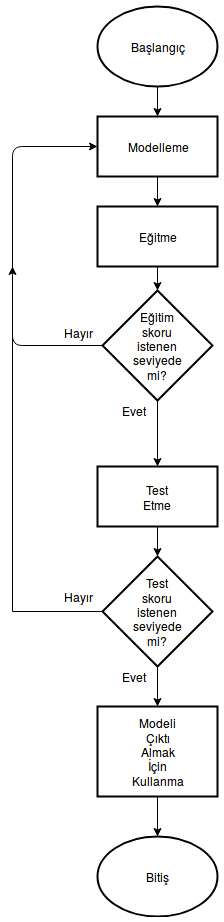
\includegraphics[width=170px]{res/fc.png}
      \end{center}
\end{document}

